\documentclass[11pt,]{report}
\usepackage{lmodern}
\usepackage{amssymb,amsmath}
\usepackage{ifxetex,ifluatex}
\usepackage{fixltx2e} % provides \textsubscript
\ifnum 0\ifxetex 1\fi\ifluatex 1\fi=0 % if pdftex
  \usepackage[T1]{fontenc}
  \usepackage[utf8]{inputenc}
\else % if luatex or xelatex
  \ifxetex
    \usepackage{mathspec}
  \else
    \usepackage{fontspec}
  \fi
  \defaultfontfeatures{Ligatures=TeX,Scale=MatchLowercase}
    \setmainfont[]{Lato}
    \setmonofont[Mapping=tex-ansi,Scale=0.7]{Hack}
\fi
% use upquote if available, for straight quotes in verbatim environments
\IfFileExists{upquote.sty}{\usepackage{upquote}}{}
% use microtype if available
\IfFileExists{microtype.sty}{%
\usepackage{microtype}
\UseMicrotypeSet[protrusion]{basicmath} % disable protrusion for tt fonts
}{}
\usepackage[a4paper,left=2.5cm,right=2.5cm,top=3cm,bottom=3cm]{geometry}
\usepackage{hyperref}
\PassOptionsToPackage{usenames,dvipsnames}{color} % color is loaded by hyperref
\hypersetup{unicode=true,
            pdftitle={Lending Club},
            pdfauthor={Emmanuel Rialland - https://github.com/Emmanuel\_R8},
            colorlinks=true,
            linkcolor=Maroon,
            citecolor=Blue,
            urlcolor=Blue,
            breaklinks=true}
\urlstyle{same}  % don't use monospace font for urls
\usepackage{natbib}
\bibliographystyle{apalike}
\usepackage{color}
\usepackage{fancyvrb}
\newcommand{\VerbBar}{|}
\newcommand{\VERB}{\Verb[commandchars=\\\{\}]}
\DefineVerbatimEnvironment{Highlighting}{Verbatim}{commandchars=\\\{\}}
% Add ',fontsize=\small' for more characters per line
\usepackage{framed}
\definecolor{shadecolor}{RGB}{248,248,248}
\newenvironment{Shaded}{\begin{snugshade}}{\end{snugshade}}
\newcommand{\AlertTok}[1]{\textcolor[rgb]{0.94,0.16,0.16}{#1}}
\newcommand{\AnnotationTok}[1]{\textcolor[rgb]{0.56,0.35,0.01}{\textbf{\textit{#1}}}}
\newcommand{\AttributeTok}[1]{\textcolor[rgb]{0.77,0.63,0.00}{#1}}
\newcommand{\BaseNTok}[1]{\textcolor[rgb]{0.00,0.00,0.81}{#1}}
\newcommand{\BuiltInTok}[1]{#1}
\newcommand{\CharTok}[1]{\textcolor[rgb]{0.31,0.60,0.02}{#1}}
\newcommand{\CommentTok}[1]{\textcolor[rgb]{0.56,0.35,0.01}{\textit{#1}}}
\newcommand{\CommentVarTok}[1]{\textcolor[rgb]{0.56,0.35,0.01}{\textbf{\textit{#1}}}}
\newcommand{\ConstantTok}[1]{\textcolor[rgb]{0.00,0.00,0.00}{#1}}
\newcommand{\ControlFlowTok}[1]{\textcolor[rgb]{0.13,0.29,0.53}{\textbf{#1}}}
\newcommand{\DataTypeTok}[1]{\textcolor[rgb]{0.13,0.29,0.53}{#1}}
\newcommand{\DecValTok}[1]{\textcolor[rgb]{0.00,0.00,0.81}{#1}}
\newcommand{\DocumentationTok}[1]{\textcolor[rgb]{0.56,0.35,0.01}{\textbf{\textit{#1}}}}
\newcommand{\ErrorTok}[1]{\textcolor[rgb]{0.64,0.00,0.00}{\textbf{#1}}}
\newcommand{\ExtensionTok}[1]{#1}
\newcommand{\FloatTok}[1]{\textcolor[rgb]{0.00,0.00,0.81}{#1}}
\newcommand{\FunctionTok}[1]{\textcolor[rgb]{0.00,0.00,0.00}{#1}}
\newcommand{\ImportTok}[1]{#1}
\newcommand{\InformationTok}[1]{\textcolor[rgb]{0.56,0.35,0.01}{\textbf{\textit{#1}}}}
\newcommand{\KeywordTok}[1]{\textcolor[rgb]{0.13,0.29,0.53}{\textbf{#1}}}
\newcommand{\NormalTok}[1]{#1}
\newcommand{\OperatorTok}[1]{\textcolor[rgb]{0.81,0.36,0.00}{\textbf{#1}}}
\newcommand{\OtherTok}[1]{\textcolor[rgb]{0.56,0.35,0.01}{#1}}
\newcommand{\PreprocessorTok}[1]{\textcolor[rgb]{0.56,0.35,0.01}{\textit{#1}}}
\newcommand{\RegionMarkerTok}[1]{#1}
\newcommand{\SpecialCharTok}[1]{\textcolor[rgb]{0.00,0.00,0.00}{#1}}
\newcommand{\SpecialStringTok}[1]{\textcolor[rgb]{0.31,0.60,0.02}{#1}}
\newcommand{\StringTok}[1]{\textcolor[rgb]{0.31,0.60,0.02}{#1}}
\newcommand{\VariableTok}[1]{\textcolor[rgb]{0.00,0.00,0.00}{#1}}
\newcommand{\VerbatimStringTok}[1]{\textcolor[rgb]{0.31,0.60,0.02}{#1}}
\newcommand{\WarningTok}[1]{\textcolor[rgb]{0.56,0.35,0.01}{\textbf{\textit{#1}}}}
\usepackage{longtable,booktabs}
\usepackage{graphicx,grffile}
\makeatletter
\def\maxwidth{\ifdim\Gin@nat@width>\linewidth\linewidth\else\Gin@nat@width\fi}
\def\maxheight{\ifdim\Gin@nat@height>\textheight\textheight\else\Gin@nat@height\fi}
\makeatother
% Scale images if necessary, so that they will not overflow the page
% margins by default, and it is still possible to overwrite the defaults
% using explicit options in \includegraphics[width, height, ...]{}
\setkeys{Gin}{width=\maxwidth,height=\maxheight,keepaspectratio}
\IfFileExists{parskip.sty}{%
\usepackage{parskip}
}{% else
\setlength{\parindent}{0pt}
\setlength{\parskip}{6pt plus 2pt minus 1pt}
}
\setlength{\emergencystretch}{3em}  % prevent overfull lines
\providecommand{\tightlist}{%
  \setlength{\itemsep}{0pt}\setlength{\parskip}{0pt}}
\setcounter{secnumdepth}{5}
% Redefines (sub)paragraphs to behave more like sections
\ifx\paragraph\undefined\else
\let\oldparagraph\paragraph
\renewcommand{\paragraph}[1]{\oldparagraph{#1}\mbox{}}
\fi
\ifx\subparagraph\undefined\else
\let\oldsubparagraph\subparagraph
\renewcommand{\subparagraph}[1]{\oldsubparagraph{#1}\mbox{}}
\fi

%%% Use protect on footnotes to avoid problems with footnotes in titles
\let\rmarkdownfootnote\footnote%
\def\footnote{\protect\rmarkdownfootnote}

%%% Change title format to be more compact
\usepackage{titling}

% Create subtitle command for use in maketitle
\providecommand{\subtitle}[1]{
  \posttitle{
    \begin{center}\large#1\end{center}
    }
}

\setlength{\droptitle}{-2em}

  \title{Lending Club}
    \pretitle{\vspace{\droptitle}\centering\huge}
  \posttitle{\par}
  \subtitle{HarvardX - PH125.9x Data Science Capstone}
  \author{Emmanuel Rialland - \url{https://github.com/Emmanuel_R8}}
    \preauthor{\centering\large\emph}
  \postauthor{\par}
      \predate{\centering\large\emph}
  \postdate{\par}
    \date{November 03, 2019}

% Additional packages for Kable Extra
\usepackage{caption}
\usepackage{float}
\usepackage{array}
\usepackage{booktabs}
\usepackage{longtable}
\usepackage{multirow}
\usepackage{wrapfig}
\usepackage{colortbl}
\usepackage{pdflscape}
\usepackage{tabu}
\usepackage{threeparttable}
\usepackage{threeparttablex}
\usepackage[normalem]{ulem}
\usepackage{makecell}
%
\usepackage{amsthm}
\makeatletter
\def\thm@space@setup{%
  \thm@preskip=8pt plus 2pt minus 4pt
  \thm@postskip=\thm@preskip
}
\makeatother

\begin{document}
\maketitle

{
\hypersetup{linkcolor=black}
\setcounter{tocdepth}{2}
\tableofcontents
}
\listoftables
\listoffigures
\small

\normalsize

\small

\normalsize

\small

\normalsize

\small

\normalsize

\small

\normalsize

\small

\normalsize

\hypertarget{introduction}{%
\chapter*{Introduction}\label{introduction}}
\addcontentsline{toc}{chapter}{Introduction}

Lending Club (\emph{LC}) is an American company listed on the New York stock exchange that provides a platform for peer-to-peer lending. Unlike banks, it does not take deposits and invest them. It is purely a matching system. Each loan is split into \$25 that multiple investors can invest in. LC is remunerated by fees received from both sides. LC states that they have intermediated more than \$50bln since they started operations. Further description of the company is easily available online numerous sources.

In order for investors to make the best investment decisions, LC make a historical dataset publicly available to all registered investors. This dataset is the subject of this report. It was downloaded from the Kaggle data science website\footnote{\url{https://www.kaggle.com/wendykan/lending-club-loan-data/data}}.

The size of the dataset is rich enough that it could be used to answer many different questions. We decided for a focused approach. Following Chapter 5 of \citep{peng2012exploratory}, we will first formulate the question we want to answer to guide our analysis.

The business model of LC is to match borrowers and investors. Naturally, more people want to receive money than part with it. An important limiting factor to LC's growth is the ability to attract investors, build a trusting relationship where, as a minimum first step, investors trust LC to provide accurate, transparent and reliable information of the borrowers. For this purpose, LC decided not only to provide extensive information about potential borrowers' profile, but also historical information about past borrowers' performance. This is, as we understand, one of the key purposes of this dataset. We decided to use the dataset for this very purpose. Essentially, the questions are: \textbf{given a borrower profile, is his/her rating appropriate in terms of risk of default? And if a default occurs, what is the expected recovery? The summary question is: given a borrower profile, is the risk/reward balance appropriate to commit funds?} In answering this question, we understand that LC allows investment of very granular amounts. Therefore, even an individual investor can diversify his/her loan and risk portfolio. It is not necessary to `gamble' funds on a single borrower. This is exactly what institutional investors achieve through syndication (although on a very different scale, typically \$10-25mln for a medium-size bank).

For this exercise, we made two simplifying (hopefully not simplistic) assumptions:

\begin{itemize}
\item
  In determining the risk/return balance, we have not accounted for LC's cost of intermediation. By ignoring fees paid by both sides, we obviously overestimate the returns to the investors. But in first approximation, \textbf{we will assume that the risk/reward balance, from the investors' point of view, across ratings is independent from fees.} This is a simplification. Real-world fees are higher the lower the investment grade and push the investors to receive, and the borrowers to pay, higher interest margin.
\item
  All-in interest rates paid by borrowers are fixed. This is highly desirable for borrowers to be able to manage their cashflow. However, an investor should always consider an investment return as a margin above a risk-free return. Banks would look at LIBOR; bond investors (e.g.~life insurers) would look at government bonds. Those risk-free rates can change very quickly, whereas we understand that LC sets those rates on a less frequent basis. In other word, the risk premium will vary rapidly. \textbf{We assume that individual investors are `in-elastic' to change in implied risk premia.} But we recognise this as a limitation of our work.
\end{itemize}

This report is organised as follows:

\begin{itemize}
\tightlist
\item
  {[}XXXX{]}
\end{itemize}

\hypertarget{dataset}{%
\chapter{Dataset}\label{dataset}}

The data is sourced as a \emph{SQLite} database that was imported as a \texttt{dataframe} with the \texttt{RSQLite} package. The variables were reformatted according to their respective types.

We also sourced US zip and FIPS codes, and macroeconomical data for possible geographical statistics. The source code for the data import and reformatting is given in appendix.

\hypertarget{preamble}{%
\section{Preamble}\label{preamble}}

The LendingClub dataset, although rich, is difficult to interpret. The only explanation of what the variables mean comes from a spreadsheet attached to the dataset. The explanations are not precise and/or subject to conflicting interpretation. Despite serching the LendingClub website, no further original information was found. We collected a number of reasonable assumptions in Appendix.

The dataset has been used a number of times in the past by various people. One paper \citep{kim2019ensemble} mentions they used a dataset that included 110 variables, which is less than ours with 145 variables. The dataset has changed over time in ways we do not know.

\hypertarget{general-presentation}{%
\section{General presentation}\label{general-presentation}}

The original dataset is rich: it includes 2260668 loan samples, each containing 144 variables (after the identification variables filled with null values). The loans were issued from 2007-06-01 to 2018-12-01.

\hypertarget{business-volume}{%
\subsection{Business volume}\label{business-volume}}

The dataset represents a total of ca.\$34bln in loan principals, which is a substantial share of the total amount stated to have been intermediated to date by LC (reported to be \$50bln+). About 60\% of the portfolio is fully repaid. See Table \ref{tab:loan-per-status}.

\small

\begin{table}

\caption{\label{tab:loan-per-status}Number of loans per status}
\centering
\begin{tabular}[t]{>{\raggedright\arraybackslash}p{8.5cm}>{\raggedleft\arraybackslash}p{2.5cm}>{\raggedleft\arraybackslash}p{3.5cm}}
\toprule
Loan status & Count & Proportion (\%)\\
\midrule
Charged Off & 261655 & 11.574\\
Current & 919695 & 40.682\\
Default & 31 & 0.001\\
Does not meet the credit policy. Status:Charged Off & 761 & 0.034\\
Does not meet the credit policy. Status:Fully Paid & 1988 & 0.088\\
\addlinespace
Fully Paid & 1041952 & 46.090\\
In Grace Period & 8952 & 0.396\\
Late (16-30 days) & 3737 & 0.165\\
Late (31-120 days) & 21897 & 0.969\\
\bottomrule
\end{tabular}
\end{table}

\normalsize

Figure \ref{fig:business-volume-per-month} plots the number, volume (cumulative principal amount) and average principal per loan. It shows that the business grew exponentially (in the common sense of the word) from inception until 2016. At this point, according to Wikipedia \footnote{source: \url{https://en.wikipedia.org/wiki/LendingClub} - Retrieval date 15 September 2019}:

" \emph{Like other peer-to-peer lenders including Prosper, Sofi and Khutzpa.com, LendingClub experienced increasing difficulty attracting investors during early 2016. This led the firm to increase the interest rate it charges borrowers on three occasions during the first months of the year. The increase in interest rates and concerns over the impact of the slowing United States economy caused a large drop in LendingClub's share price.}"

The number and volume of loans plotted have been aggregated by month. The growth is very smooth in the early years, and suddenly very volatile. As far as the first part of the dataset is concerned, a starting business could expect to be volatile and could witness a yearly cycle (expected from economic consumption figures) superimposed on the growth trend. This is not the case.

An interesting metric is that the average principal of loans has increased (see Figure \ref{business-volume-per-month}, on a sample of 100,000 loans). Partly, the increase in the early years could be interpreted success in confidence building. This metric plateau-ed in 2016 and decreased afterwards, but to a much lesser extent than the gross volume metrics. However, it is more volatile than the two previous metrics in the early years.

By the end of the dataset, all metrics have essentially recovered to their 2016 level.

\hypertarget{loan-lifecyle-and-status}
\end{Highlighting}
\end{Shaded}

\normalsize

The dataset describes the life cycle of a loan. In the typical (ideal) case, we understand it to be:

\[ 
\text{Loan is approved}  \rightarrow  \text{Full amount funded by investors} \rightarrow \text{Loan marked as Current} \rightarrow \text{Fully Paid}
\]

In the worst case, it is:

\[ 
\text{Loan is approved}  \rightarrow  \text{Full amount funded by investors} \rightarrow \text{Loan marked as Current} \rightarrow 
\]

\[
\rightarrow \text{Grace period (missed payments under 2 weeks)} \rightarrow \text{Late 15 to 31 days} \rightarrow
\]

\[
\rightarrow  \text{Late 31 to 120 days} \rightarrow  \text{Default} \rightarrow  \text{Charged Off}
\]

Note that \emph{Default} precedes and is distinct from \emph{Charged Off} \footnote{See LendingClub FAQ at \url{https://help.lendingclub.com/hc/en-us/articles/215488038}}. A couple of things could happen to a loan in default:

\begin{itemize}
\item
  LC and the borrower restructure the loan with a new repayment schedule, where the borrower may repay a lesser amount over a longer period; or,
\item
  the claim could be sold to a debt recovery company that would buy the claim from LC/investors. This would be the final payment (if any) received by LC and the investors.
\end{itemize}

The dataset also describes situations where a borrower negotiated a restructuring of the repayment schedule in case of unexpected hardship (e.g.~disaster, sudden unemployment).

Note that this progression of distinguishing default (event in time) and actual financial loss mirrors what banks and rating agencies do\textgreater{} The former is called the \emph{Probability of Default} (PD), the latter \emph{Loss Given Default} (LGD). Ratings change over time (in a process resembling a Markov Chains). LGD show some correlations with ratings. The dataset, although detailed, does not include the full life of each loan to conduct this sort of analysis (change of loan quality over time). This is an important reason why we decided to focus on the loan approval and expected return.

\hypertarget{loan-application}{%
\subsection{Loan application}\label{loan-application}}

Before a loan is approved, the borrower undergoes a review process that assess his/her capacity to repay. This includes:

\begin{itemize}
\item
  employment situation and income, as well whether this income and possibly its source has been independently verified;
\item
  whether the application is made jointly (likely with a partner or a spouse, but there are no details);
\item
  housing situation (owner, owner with current mortgage, rental) and in which county he/she lives (that piece of information is partially anonymised by removing the last 2 digits of the borrower's zipcode);
\item
  the amount sought, its tenor and the purpose of the loan; and,
\item
  what seems to be previous credit history (number of previous deliquencies). The dataset is very confusing in that regard: it is clear that such information relates to before the loan is approved in the case of the joint applicant. In the case of the principal borrower however, the variable descriptions could be read as pre-approval information, or information gathered during the life of the loan. We have assumed that the information related to the principal borrower is also pre-approval. We also used \emph{Sales Supplements} from the LC website\footnote{See \url{https://www.lendingclub.com/legal/prospectus}} that describe some of the information provided to investors. LendingClub also provides a summary description of its approval process in its regulatory filings with the Securities Exchange Commission \citep{LC201908S3}.
\end{itemize}

\hypertarget{interest-rates}{%
\subsection{Interest rates}\label{interest-rates}}

Based on this information, the loan is approved or not. Approval includes the final amount (which could be lower than the amount requested), tenor (3 or 5 years) and a rating similar to those given to corporate borrowers. Unlike corporate borrowers however, the rating mechanically determines the rate of interest according to a grid known to the borrower in advance\footnote{\url{https://www.lendingclub.com/investing/investor-education/interest-rates-and-fees}}. The rates have changed over time. Those changes where not as frequent as market conditions (e.g.~changes in Federal Reserve Bank's rates)\footnote{Corporate borrowers would negociate interest margins on a case-by-case basis despite similar risk profiles.}.

Figure \ref{fig:interest-rate-table} \footnote{source: \url{https://www.lendingclub.com/investing/investor-education/interest-rates-and-fees}} shows the predetermined interest rate depending on the initial rating as of July 2019.

\small

\begin{figure}

{\centering 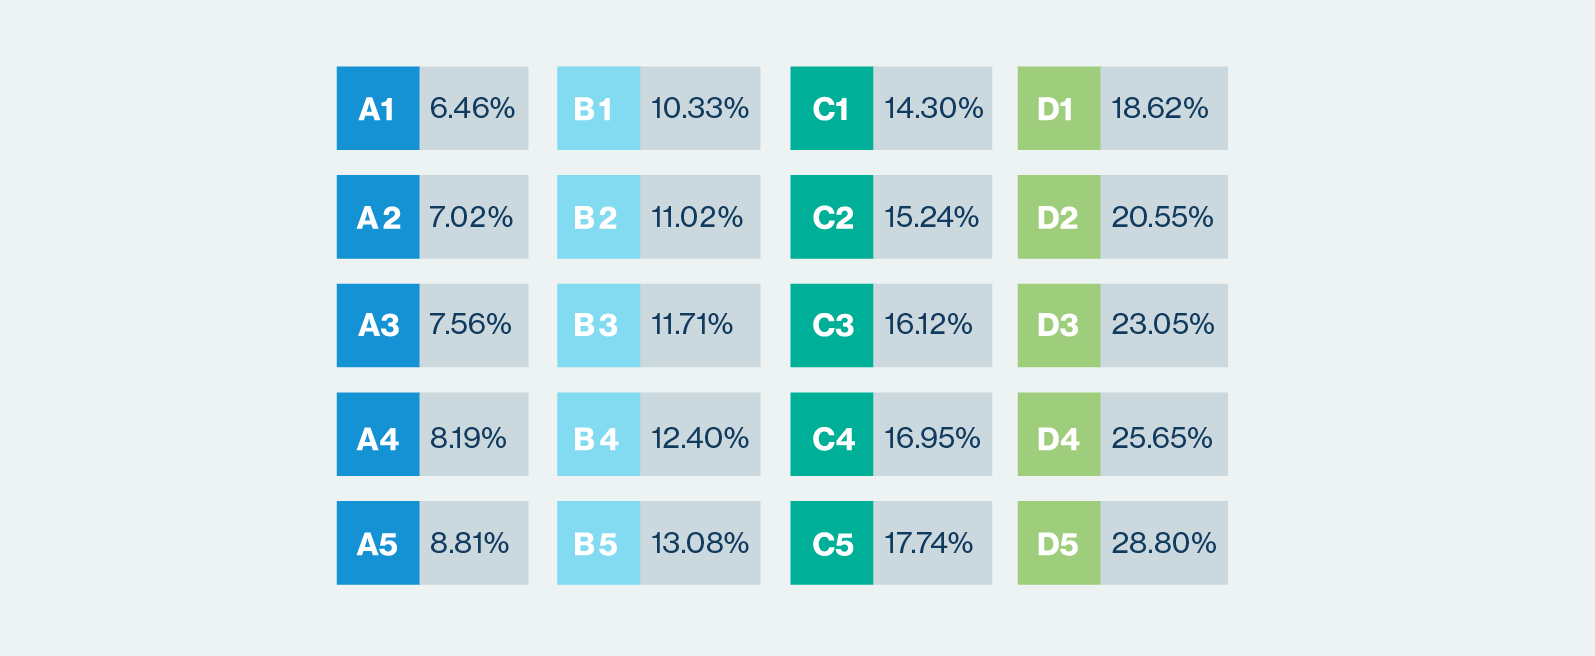
\includegraphics[width=0.7\linewidth]{images/interest-rates-jul2019} 

}

\caption{Interest rates given rating}\label{fig:interest-rate-table}
\end{figure}

\normalsize

At the date of this report, the ratings range from \texttt{A} (the best) down to \texttt{D}, each split in 5 sub-ratings. However, LC previously also intermediated loans rated F or G (until 6 November 2017) and E (until 30 June 2019) \footnote{See \url{https://www.lendingclub.com/info/demand-and-credit-profile.action}}. This explains that such ratings are in the dataset. We will assume that the ratings in the dataset are the rating at the time of approval and that, even if loans are re-rated by LC, the dataset does not reflect it.

Figures \ref{fig:interest-over-time} shows the change in interest rate over time for different ratings and separated for each tenor. (Each figure is on a sample of 100,000 loans.) For each rating, we can see several parallel lines which correspond to the 5 sub-rating of each rating. We note that the range of interest rates has substantial widened over time. That is, the risk premium necessary to attract potential investors has had to substantially increase. In the most recent years, the highest rates exceed 30\% which is higher than many credit cards.3-year loans are, unsurprinsingly, considered safer (more A-rated, less G-rated). Identical ratings attract identical rates of interest.

\small

\begin{figure}

{\centering \includegraphics[width=0.7\linewidth]{HarvardX-LendingClub_files/figure-latex/interest-over-time-1} 

}

\caption{Interest rate per grade over time}\label{fig:interest-over-time}
\end{figure}

\normalsize

By comparison, we plot the 3-year (in red) and 5-year (in blue) bank swap rates in Figure @(fig:swap-rates). We see that the swap curve has flattened in recent times (3-year and 5-y rates are almost identical). We also can see that in broad terms the interest rates charged reflect those underlying swap rates. It is therefore most relevant to examine the credit margins added to the swap rates.

\small

\begin{figure}

{\centering \includegraphics[width=0.7\linewidth]{HarvardX-LendingClub_files/figure-latex/swap-rates-1} 

}

\caption{Historical Swap Rates}\label{fig:swap-rates}
\end{figure}

\normalsize

Figures \ref{fig:margin-over-time} shows the change in credit margin over time for different ratings and separated for each tenor. (Each figure is on a sample of 100,000 loans.) As above, for each rating, we can see several parallel lines which correspond to the 5 sub-rating of each rating. We note that the range of credit margins has widened over time but less than the interest rates. Identical ratings attract identical credit margins.

\small

\begin{figure}

{\centering \includegraphics[width=0.7\linewidth]{HarvardX-LendingClub_files/figure-latex/margin-over-time-1} 

}

\caption{Credit margins per grade over time}\label{fig:margin-over-time}
\end{figure}

\normalsize

{[}TODO: DTI, amount\ldots{} by grade{]}

\hypertarget{payments}{%
\subsection{Payments}\label{payments}}

The loans are approved for only two tenors, 3 and 5 years, with monthly repayments. Installments are calculated easily with the usual formula:

\[
Installment = Principal \times \frac{1}{1 - \frac{1}{(1+rate)^N}}
\]

Where \(Principal\) is the amount borrowed, \(rate = \frac{\text{Quoted Interest Rate}}{12}\) is the monthly interest rate, and \(N\) is the number of installments (36 or 60 monthly payments). The following piece of code shows that the average error between this formula and the dataset value is about 2 cents. We therefore precisely understand this variable.

\small

\begin{Shaded}
\begin{Highlighting}[numbers=left,,]
\KeywordTok{local}\NormalTok{(\{}
\NormalTok{  installmentError <-}\StringTok{ }\NormalTok{loans }\OperatorTok
\StringTok{    }\KeywordTok{mutate}\NormalTok{(}
      \DataTypeTok{PMT =} \KeywordTok{round}\NormalTok{(funded_amnt }\OperatorTok{*}\StringTok{ }\NormalTok{int_rate }\OperatorTok{/}\StringTok{ }\DecValTok{12} \OperatorTok{/}\StringTok{ }\NormalTok{(}\DecValTok{1} \OperatorTok{-}\StringTok{ }\DecValTok{1} \OperatorTok{/}\StringTok{ }\NormalTok{(}\DecValTok{1} \OperatorTok{+}\StringTok{ }\NormalTok{int_rate }\OperatorTok{/}\StringTok{ }\DecValTok{12}\NormalTok{) }\OperatorTok{^}
\StringTok{                                                   }\NormalTok{term), }\DecValTok{2}\NormalTok{),}
      \DataTypeTok{PMT_delta =} \KeywordTok{abs}\NormalTok{(installment }\OperatorTok{-}\StringTok{ }\NormalTok{PMT)}
\NormalTok{    ) }\OperatorTok
\StringTok{    }\KeywordTok{select}\NormalTok{(PMT_delta)}
  
  \KeywordTok{mean}\NormalTok{(}\DecValTok{100} \OperatorTok{*}\StringTok{ }\NormalTok{installmentError}\OperatorTok{$}\NormalTok{PMT_delta)}
\NormalTok{\})}
\end{Highlighting}
\end{Shaded}

\normalsize

\hypertarget{variables}{%
\section{Variables}\label{variables}}

We here present the dataset in a bit more details The full list of variable is given in appendix (see Table \ref{tab:variable-description}). This dataset will be reduced as we focused on our core question: \emph{Are LC's loans priced appropriately?}.

\hypertarget{general}{%
\subsection{General}\label{general}}

\small

\begin{figure}

{\centering \includegraphics[width=0.7\linewidth]{HarvardX-LendingClub_files/figure-latex/business-volume-per-month-1} 

}

\caption{Business volume written per month}\label{fig:business-volume-per-month}
\end{figure}

\normalsize

\hypertarget{identification}{%
\subsection{Identification}\label{identification}}

The dataset is anonymised (all identifying ID numbers are deleted) and we therefore removed those columns from the dataset. Since the identification \texttt{ID}s have been removed to anonymise the dataset, we cannot see if a borrower borrowed several times.

\hypertarget{loan-decision}{%
\section{Loan decision}\label{loan-decision}}

As indicated in the introduction, our focus is on loans that have gone through their entire life cycle to consider their respective pricing, risk and profitability. To that effect, we will remove all loans which are still current (either performing or not). From here on, everything will be based on this reduced dataset.

In this reduced dataset, we focus on loans that have matured or been terminated. It contains 1306356 samples. Most of the loans (ca.80\%) have been repaid in full. See Table \ref{tab:matured-loans}.

\small

\begin{table}

\caption{\label{tab:matured-loans}Matured loans per status}
\centering
\begin{tabular}[t]{>{\raggedright\arraybackslash}p{6cm}>{\raggedleft\arraybackslash}p{4cm}r}
\toprule
Loan status & Count & Proportion (\%)\\
\midrule
Fully Paid & 1041952 & 26048800\\
Charged Off & 261655 & 6541375\\
Does not meet the credit policy. Status:Fully Paid & 1988 & 49700\\
Does not meet the credit policy. Status:Charged Off & 761 & 19025\\
\bottomrule
\end{tabular}
\end{table}

\normalsize

When grouped by grade (Figure \ref{fig:funded-by-subgrade}), we see a clear correlation between grade and default: the lower the grade the higher the portion defaults (all the way down to about 50\%). In addition, most of the business is written in the B- or C-rating range.

\small

\begin{figure}

{\centering \includegraphics[width=0.7\linewidth]{HarvardX-LendingClub_files/figure-latex/funded-by-subgrade-1} 

}

\caption{Funding and Write-offs by Sub-grades}\label{fig:funded-by-subgrade}
\end{figure}

\normalsize

\hypertarget{modelling}{%
\chapter{Modelling}\label{modelling}}

At the outset, the dataset presents a number of challenges:

\begin{itemize}
\item
  There is a mix of continuous and categorical data.
\item
  The number of observations is very large.
\end{itemize}

The diagram \ref{fig:scikit-map}\footnote{Source: \url{https://scikit-learn.org/stable/tutorial/machine_learning_map/index.html}} shows a useful decision tree.

\small

\begin{figure}

{\centering 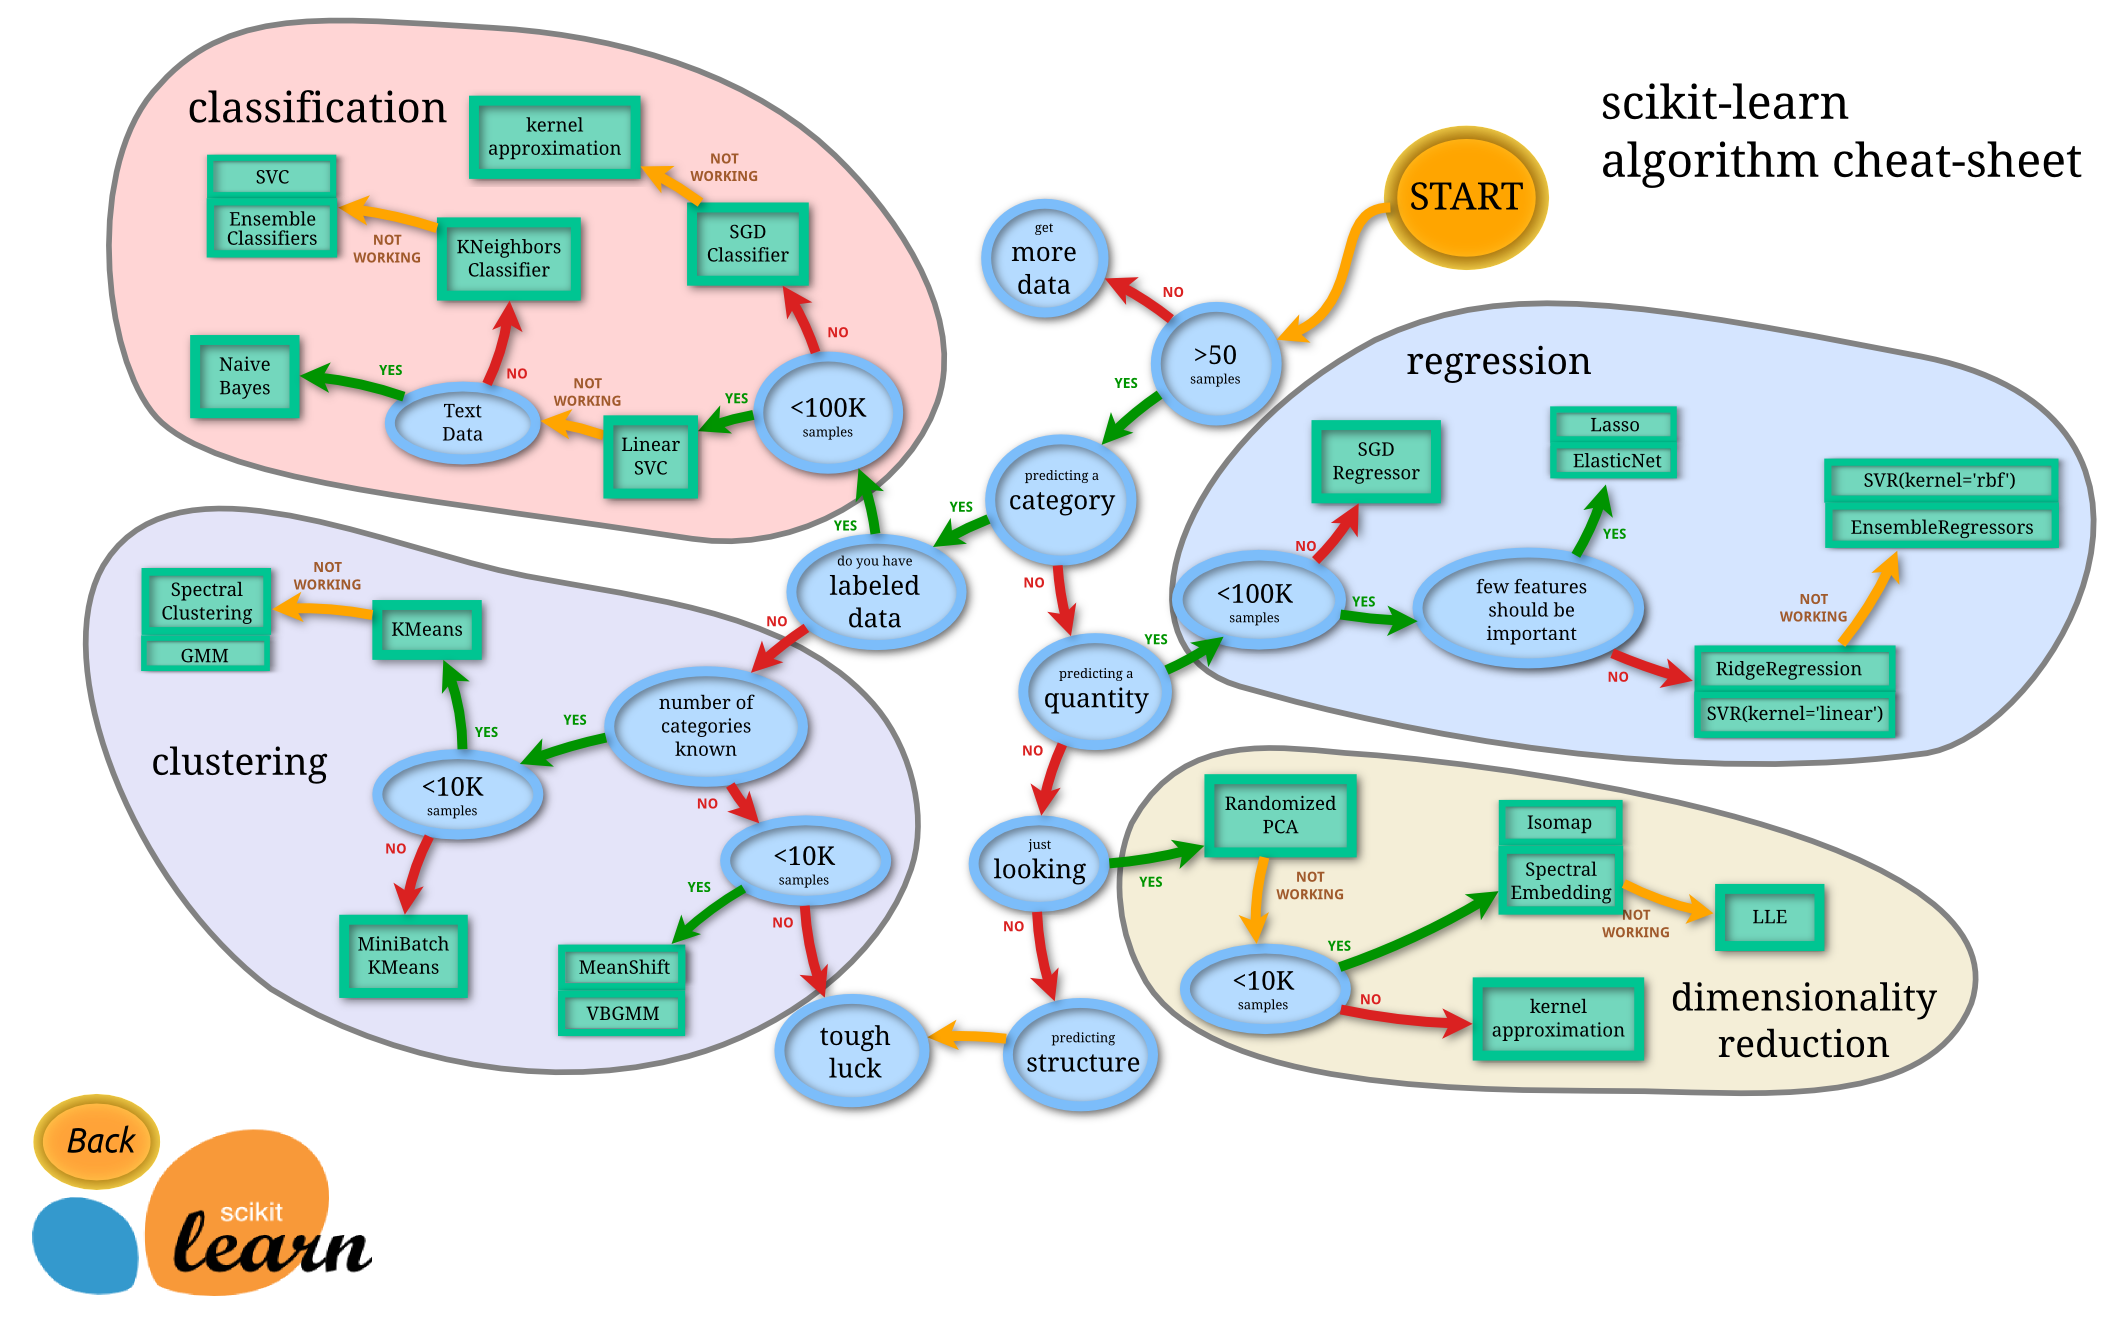
\includegraphics[width=0.7\linewidth]{images/scikit-learn-mlmap} 

}

\caption{Scikit Learn algorithm cheat-sheet}\label{fig:scikit-map}
\end{figure}

\normalsize

\hypertarget{appendix}{%
\chapter*{Appendix}\label{appendix}}
\addcontentsline{toc}{chapter}{Appendix}

\hypertarget{list-of-assumptions-limitations-regarding-the-dataset}{%
\section{List of assumptions / limitations regarding the dataset}\label{list-of-assumptions-limitations-regarding-the-dataset}}

As mentioned during this report, we had to make numerous assumptions given the lack of clarity of the variable descriptions.

\begin{itemize}
\item
  The dataset does not contain any errors that we cannot notice (e.g.~minor error of amount or rate, zipcode).
\item
  The day-1 rating is between A1 and (and no lower than) G5. No note is rated lower than E5 from 6 November 2017, and lower than D5 from 30 June 2019.
\item
  Credit history information for the principal borrower relates to pre-approval and not post-funding. This is clear for the joint applicants, but simply an assumption for the principal borrower.
\item
  \emph{Survival effect}: The dataset does not include applications that were rejected.
\end{itemize}

We do hope that LendingClub investors receive information of much better quality!

\hypertarget{data-preparation-and-formatting}{%
\section{Data preparation and formatting}\label{data-preparation-and-formatting}}

We used different sources of information:

\begin{itemize}
\item
  The LendingClub dataset made available on Kaggle;
\item
  US georgraphical data about zip and FIPS codes;
\item
  Market interest rates from the Saint Louis Federal Reserve Bank; and,
\item
  Macro data from the same source.
\end{itemize}

We here show the code used to prepare the data.

\hypertarget{lendinclub-dataset}{%
\subsection{LendinClub dataset}\label{lendinclub-dataset}}

\small

\begin{Shaded}
\begin{Highlighting}[numbers=left,,]
\KeywordTok{local}\NormalTok{(\{}
  \CommentTok{#}
  \CommentTok{# STEP 1: Download the dataset}
  \CommentTok{#}
  \CommentTok{#   Got to https://www.kaggle.com/wendykan/lending-club-loan-data}
  \CommentTok{#}
  \CommentTok{#   Download into the 'datasets' subdirectory}
  \CommentTok{#   Unzip the file.}
  \CommentTok{#   }\AlertTok{WARNING}\CommentTok{: The unzipping will be about 2.4GB}
  \CommentTok{#}
  \CommentTok{#   Name the sql database "datasets/lending_club.sqlite"}
  \CommentTok{#}
  
  \CommentTok{#}
  \CommentTok{# STEP 2: Prepare the dabase as a tibble}
  \CommentTok{#}
  
  \KeywordTok{library}\NormalTok{(RSQLite)}
\NormalTok{  db_conn <-}
\StringTok{    }\KeywordTok{dbConnect}\NormalTok{(RSQLite}\OperatorTok{::}\KeywordTok{SQLite}\NormalTok{(), }\StringTok{"datasets/lending_club.sqlite"}\NormalTok{)}
  \KeywordTok{dbListTables}\NormalTok{(db_conn)}
  
  \CommentTok{# Returns a 2.96GB data frame}
\NormalTok{  lending_club <-}\StringTok{ }\KeywordTok{dbGetQuery}\NormalTok{(db_conn, }\StringTok{"SELECT * FROM loan"}\NormalTok{)}
\NormalTok{  lending_club <-}\StringTok{ }\KeywordTok{as_tibble}\NormalTok{(lending_club)}
  
  \CommentTok{# Close the database}
  \KeywordTok{dbDisconnect}\NormalTok{(db_conn)}
  
  \CommentTok{# Compressed to ca.285MB on disk}
  \KeywordTok{saveRDS}\NormalTok{(lending_club, }\StringTok{"datasets/lending_club.rds"}\NormalTok{)}
  
  
  \KeywordTok{library}\NormalTok{(tidyverse)}
  \KeywordTok{library}\NormalTok{(lubridate)}
  \KeywordTok{library}\NormalTok{(hablar)}
  
  \CommentTok{# Before reformat in case the previous step was already done}
  \CommentTok{# lending_club <- readRDS("datasets/lending_club.rds")}
  \CommentTok{#}
  \CommentTok{# str(lending_club)}
  \CommentTok{#}
  
  \CommentTok{# We leave the original dataset untouched and work with a copy.}
\NormalTok{  lc <-}\StringTok{ }\NormalTok{lending_club}
  
\NormalTok{  lc <-}\StringTok{ }\NormalTok{lc }\OperatorTok
\StringTok{    }\CommentTok{# Remove useless strings}
\StringTok{    }\KeywordTok{mutate}\NormalTok{(}
      \DataTypeTok{term       =} \KeywordTok{str_remove}\NormalTok{(term, }\StringTok{" months"}\NormalTok{),}
      \DataTypeTok{emp_length =} \KeywordTok{str_replace}\NormalTok{(emp_length, }\StringTok{"<1"}\NormalTok{, }\StringTok{"0"}\NormalTok{),}
      \DataTypeTok{emp_length =} \KeywordTok{str_replace}\NormalTok{(emp_length, }\StringTok{"10+"}\NormalTok{, }\StringTok{"10"}\NormalTok{),}
      \DataTypeTok{emp_length =} \KeywordTok{str_remove}\NormalTok{(emp_length, }\StringTok{"years"}\NormalTok{)}
\NormalTok{    ) }\OperatorTok
\StringTok{    }
\StringTok{    }\CommentTok{# Creates dates out of strings - Parse errors will be raised when no dates.}
\StringTok{    }\KeywordTok{mutate}\NormalTok{(}
      \DataTypeTok{debt_settlement_flag_date =} \KeywordTok{as_date}\NormalTok{(}\KeywordTok{dmy}\NormalTok{(}
        \KeywordTok{str_c}\NormalTok{(}\StringTok{"1-"}\NormalTok{, debt_settlement_flag_date)}
\NormalTok{      )),}
      \DataTypeTok{earliest_cr_line          =} \KeywordTok{as_date}\NormalTok{(}\KeywordTok{dmy}\NormalTok{(}\KeywordTok{str_c}\NormalTok{(}
        \StringTok{"1-"}\NormalTok{, earliest_cr_line}
\NormalTok{      ))),}
      \DataTypeTok{hardship_start_date       =} \KeywordTok{as_date}\NormalTok{(}\KeywordTok{dmy}\NormalTok{(}\KeywordTok{str_c}\NormalTok{(}
        \StringTok{"1-"}\NormalTok{, hardship_start_date}
\NormalTok{      ))),}
      \DataTypeTok{hardship_end_date         =} \KeywordTok{as_date}\NormalTok{(}\KeywordTok{dmy}\NormalTok{(}\KeywordTok{str_c}\NormalTok{(}
        \StringTok{"1-"}\NormalTok{, hardship_end_date}
\NormalTok{      ))),}
      \DataTypeTok{issue_d                   =} \KeywordTok{as_date}\NormalTok{(}\KeywordTok{dmy}\NormalTok{(}\KeywordTok{str_c}\NormalTok{(}\StringTok{"1-"}\NormalTok{, issue_d))),}
      \DataTypeTok{last_credit_pull_d        =} \KeywordTok{as_date}\NormalTok{(}\KeywordTok{dmy}\NormalTok{(}\KeywordTok{str_c}\NormalTok{(}
        \StringTok{"1-"}\NormalTok{, last_credit_pull_d}
\NormalTok{      ))),}
      \DataTypeTok{last_pymnt_d              =} \KeywordTok{as_date}\NormalTok{(}\KeywordTok{dmy}\NormalTok{(}\KeywordTok{str_c}\NormalTok{(}
        \StringTok{"1-"}\NormalTok{, last_pymnt_d}
\NormalTok{      ))),}
      \DataTypeTok{next_pymnt_d              =} \KeywordTok{as_date}\NormalTok{(}\KeywordTok{dmy}\NormalTok{(}\KeywordTok{str_c}\NormalTok{(}
        \StringTok{"1-"}\NormalTok{, next_pymnt_d}
\NormalTok{      ))),}
      \DataTypeTok{payment_plan_start_date   =} \KeywordTok{as_date}\NormalTok{(}\KeywordTok{dmy}\NormalTok{(}\KeywordTok{str_c}\NormalTok{(}
        \StringTok{"1-"}\NormalTok{, payment_plan_start_date}
\NormalTok{      ))),}
      \DataTypeTok{sec_app_earliest_cr_line  =} \KeywordTok{as_date}\NormalTok{(}\KeywordTok{dmy}\NormalTok{(}\KeywordTok{str_c}\NormalTok{(}
        \StringTok{"1-"}\NormalTok{, sec_app_earliest_cr_line}
\NormalTok{      ))),}
      \DataTypeTok{settlement_date           =} \KeywordTok{as_date}\NormalTok{(}\KeywordTok{dmy}\NormalTok{(}\KeywordTok{str_c}\NormalTok{(}
        \StringTok{"1-"}\NormalTok{, settlement_date}
\NormalTok{      )))}
\NormalTok{    ) }\OperatorTok
\StringTok{    }
\StringTok{    }\CommentTok{# Bulk type conversion with convert from the `hablar` package}
\StringTok{    }\KeywordTok{convert}\NormalTok{(}
      \CommentTok{# Strings}
      \KeywordTok{chr}\NormalTok{(emp_title, title, url, zip_code),}
      
      \CommentTok{# Factors}
      \KeywordTok{fct}\NormalTok{(}
\NormalTok{        addr_state,}
\NormalTok{        application_type,}
\NormalTok{        debt_settlement_flag,}
\NormalTok{        desc,}
\NormalTok{        disbursement_method,}
\NormalTok{        grade,}
\NormalTok{        hardship_flag,}
\NormalTok{        hardship_loan_status,}
\NormalTok{        hardship_reason,}
\NormalTok{        hardship_status,}
\NormalTok{        hardship_type,}
\NormalTok{        home_ownership,}
\NormalTok{        id,}
\NormalTok{        initial_list_status,}
\NormalTok{        loan_status,}
\NormalTok{        member_id,}
\NormalTok{        policy_code,}
\NormalTok{        purpose,}
\NormalTok{        pymnt_plan,}
\NormalTok{        settlement_status,}
\NormalTok{        sub_grade,}
\NormalTok{        verification_status,}
\NormalTok{        verification_status_joint}
\NormalTok{      ),}
      
      \CommentTok{# Integers}
      \KeywordTok{int}\NormalTok{(}
\NormalTok{        acc_now_delinq,}
\NormalTok{        acc_open_past_24mths,}
\NormalTok{        chargeoff_within_}\DecValTok{12}\NormalTok{_mths,}
\NormalTok{        collections_}\DecValTok{12}\NormalTok{_mths_ex_med,}
\NormalTok{        deferral_term,}
\NormalTok{        delinq_2yrs,}
\NormalTok{        emp_length,}
\NormalTok{        hardship_dpd,}
\NormalTok{        hardship_length,}
\NormalTok{        inq_fi,}
\NormalTok{        inq_last_12m,}
\NormalTok{        inq_last_6mths,}
\NormalTok{        mo_sin_old_il_acct,}
\NormalTok{        mo_sin_old_rev_tl_op,}
\NormalTok{        mo_sin_rcnt_rev_tl_op,}
\NormalTok{        mo_sin_rcnt_tl,}
\NormalTok{        mort_acc,}
\NormalTok{        mths_since_last_delinq,}
\NormalTok{        mths_since_last_major_derog,}
\NormalTok{        mths_since_last_record,}
\NormalTok{        mths_since_rcnt_il,}
\NormalTok{        mths_since_recent_bc,}
\NormalTok{        mths_since_recent_bc_dlq,}
\NormalTok{        mths_since_recent_inq,}
\NormalTok{        mths_since_recent_revol_delinq,}
\NormalTok{        num_accts_ever_}\DecValTok{120}\NormalTok{_pd,}
\NormalTok{        num_actv_bc_tl,}
\NormalTok{        num_actv_rev_tl,}
\NormalTok{        num_bc_sats,}
\NormalTok{        num_bc_tl,}
\NormalTok{        num_il_tl,}
\NormalTok{        num_op_rev_tl,}
\NormalTok{        num_rev_accts,}
\NormalTok{        num_rev_tl_bal_gt_}\DecValTok{0}\NormalTok{,}
\NormalTok{        num_sats,}
\NormalTok{        num_tl_120dpd_2m,}
\NormalTok{        num_tl_30dpd,}
\NormalTok{        num_tl_90g_dpd_24m,}
\NormalTok{        num_tl_op_past_12m,}
\NormalTok{        open_acc,}
\NormalTok{        open_acc_6m,}
\NormalTok{        open_act_il,}
\NormalTok{        open_il_12m,}
\NormalTok{        open_il_24m,}
\NormalTok{        open_rv_12m,}
\NormalTok{        open_rv_24m,}
\NormalTok{        sec_app_chargeoff_within_}\DecValTok{12}\NormalTok{_mths,}
\NormalTok{        sec_app_collections_}\DecValTok{12}\NormalTok{_mths_ex_med,}
\NormalTok{        sec_app_inq_last_6mths,}
\NormalTok{        sec_app_mort_acc,}
\NormalTok{        sec_app_mths_since_last_major_derog,}
\NormalTok{        sec_app_num_rev_accts,}
\NormalTok{        sec_app_open_acc,}
\NormalTok{        sec_app_open_act_il,}
\NormalTok{        term}
\NormalTok{      ),}
      
      \CommentTok{# Floating point}
      \KeywordTok{dbl}\NormalTok{(}
\NormalTok{        all_util,}
\NormalTok{        annual_inc,}
\NormalTok{        annual_inc_joint,}
\NormalTok{        avg_cur_bal,}
\NormalTok{        bc_open_to_buy,}
\NormalTok{        bc_util,}
\NormalTok{        collection_recovery_fee,}
\NormalTok{        delinq_amnt,}
\NormalTok{        dti,}
\NormalTok{        dti_joint,}
\NormalTok{        funded_amnt,}
\NormalTok{        funded_amnt_inv,}
\NormalTok{        hardship_amount,}
\NormalTok{        hardship_last_payment_amount,}
\NormalTok{        hardship_payoff_balance_amount,}
\NormalTok{        il_util,}
\NormalTok{        installment,}
\NormalTok{        int_rate,}
\NormalTok{        last_pymnt_amnt,}
\NormalTok{        loan_amnt,}
\NormalTok{        max_bal_bc,}
\NormalTok{        orig_projected_additional_accrued_interest,}
\NormalTok{        out_prncp,}
\NormalTok{        out_prncp_inv,}
\NormalTok{        pct_tl_nvr_dlq,}
\NormalTok{        percent_bc_gt_}\DecValTok{75}\NormalTok{,}
\NormalTok{        pub_rec,}
\NormalTok{        pub_rec_bankruptcies,}
\NormalTok{        recoveries,}
\NormalTok{        revol_bal,}
\NormalTok{        revol_bal_joint,}
\NormalTok{        revol_util,}
\NormalTok{        sec_app_revol_util,}
\NormalTok{        settlement_amount,}
\NormalTok{        settlement_percentage,}
\NormalTok{        tax_liens,}
\NormalTok{        tot_coll_amt,}
\NormalTok{        tot_cur_bal,}
\NormalTok{        tot_hi_cred_lim,}
\NormalTok{        total_acc,}
\NormalTok{        total_bal_ex_mort,}
\NormalTok{        total_bal_il,}
\NormalTok{        total_bc_limit,}
\NormalTok{        total_cu_tl,}
\NormalTok{        total_il_high_credit_limit,}
\NormalTok{        total_pymnt,}
\NormalTok{        total_pymnt_inv,}
\NormalTok{        total_rec_int,}
\NormalTok{        total_rec_late_fee,}
\NormalTok{        total_rec_prncp,}
\NormalTok{        total_rev_hi_lim}
\NormalTok{      )}
\NormalTok{    ) }\OperatorTok
\StringTok{    }
\StringTok{    }\CommentTok{# Converts some values to 1/-1 (instead of Boolean)}
\StringTok{    }\KeywordTok{mutate}\NormalTok{(}
      \DataTypeTok{pymnt_plan =}           \KeywordTok{if_else}\NormalTok{(pymnt_plan }\OperatorTok{==}\StringTok{ "y"}\NormalTok{,           }\DecValTok{1}\NormalTok{, }\DecValTok{-1}\NormalTok{),}
      \DataTypeTok{hardship_flag =}        \KeywordTok{if_else}\NormalTok{(hardship_flag }\OperatorTok{==}\StringTok{ "Y"}\NormalTok{,        }\DecValTok{1}\NormalTok{, }\DecValTok{-1}\NormalTok{),}
      \DataTypeTok{debt_settlement_flag =} \KeywordTok{if_else}\NormalTok{(debt_settlement_flag }\OperatorTok{==}\StringTok{ "Y"}\NormalTok{, }\DecValTok{1}\NormalTok{, }\DecValTok{-1}\NormalTok{)}
\NormalTok{    ) }\OperatorTok
\StringTok{    }
\StringTok{    }\CommentTok{# Some values are percentages}
\StringTok{    }\KeywordTok{mutate}\NormalTok{(}
      \DataTypeTok{int_rate =}\NormalTok{ int_rate }\OperatorTok{/}\StringTok{ }\DecValTok{100}\NormalTok{,}
      \DataTypeTok{dti =}\NormalTok{ dti }\OperatorTok{/}\StringTok{ }\DecValTok{100}\NormalTok{,}
      \DataTypeTok{dti_joint =}\NormalTok{ dti_joint }\OperatorTok{/}\StringTok{ }\DecValTok{100}\NormalTok{,}
      \DataTypeTok{revol_util =}\NormalTok{ revol_util }\OperatorTok{/}\StringTok{ }\DecValTok{100}\NormalTok{,}
      \DataTypeTok{il_util =}\NormalTok{ il_util }\OperatorTok{/}\StringTok{ }\DecValTok{100}\NormalTok{,}
      \DataTypeTok{all_util =}\NormalTok{ all_util }\OperatorTok{/}\StringTok{ }\DecValTok{100}\NormalTok{,}
      \DataTypeTok{bc_open_to_buy =}\NormalTok{ bc_util }\OperatorTok{/}\StringTok{ }\DecValTok{100}\NormalTok{,}
      \DataTypeTok{pct_tl_nvr_dlq =}\NormalTok{ pct_tl_nvr_dlq }\OperatorTok{/}\StringTok{ }\DecValTok{100}\NormalTok{,}
      \DataTypeTok{percent_bc_gt_75 =}\NormalTok{ percent_bc_gt_}\DecValTok{75} \OperatorTok{/}\StringTok{ }\DecValTok{100}\NormalTok{,}
      \DataTypeTok{sec_app_revol_util =}\NormalTok{ sec_app_revol_util }\OperatorTok{/}\StringTok{ }\DecValTok{100}
\NormalTok{    ) }\OperatorTok
\StringTok{    }
\StringTok{    }\CommentTok{# Create quasi-centered numerical grades out of grade factors with "A" = 3 down to "G" = -3}
\StringTok{    }\KeywordTok{mutate}\NormalTok{(}\DataTypeTok{grade_num =} \DecValTok{4} \OperatorTok{-}\StringTok{ }\KeywordTok{as.integer}\NormalTok{(grade)) }\OperatorTok
\StringTok{    }
\StringTok{    }\CommentTok{# Ditto with sub_grades. "A1" = +3.4, "A3" = +3.0, down to "G3" = -3.0, "G5" = -3.4}
\StringTok{    }\KeywordTok{mutate}\NormalTok{(}\DataTypeTok{sub_grade_num =} \FloatTok{3.6} \OperatorTok{-}\StringTok{ }\KeywordTok{as.integer}\NormalTok{(sub_grade) }\OperatorTok{/}\StringTok{ }\DecValTok{5}\NormalTok{) }\OperatorTok
\StringTok{    }
\StringTok{    }\CommentTok{# Keep the first 3 digits of the zipcode as numbers}
\StringTok{    }\KeywordTok{mutate}\NormalTok{(}\DataTypeTok{zip_code =} \KeywordTok{as.integer}\NormalTok{(}\KeywordTok{str_sub}\NormalTok{(zip_code, }\DecValTok{1}\NormalTok{, }\DecValTok{3}\NormalTok{))) }\OperatorTok
\StringTok{    }
\StringTok{    }\CommentTok{# Remove empty columns}
\StringTok{    }\KeywordTok{select}\NormalTok{(}\OperatorTok{-}\NormalTok{id, }\OperatorTok{-}\NormalTok{member_id, }\OperatorTok{-}\NormalTok{url)}
  
  \KeywordTok{saveRDS}\NormalTok{(lc, }\StringTok{"datasets/lending_club_reformatted.rds"}\NormalTok{)}
  
  
  \CommentTok{# Select loans which have matured or been terminated}
\NormalTok{  past_loans <-}\StringTok{ }\NormalTok{lc }\OperatorTok
\StringTok{    }\KeywordTok{filter}\NormalTok{(}
\NormalTok{      loan_status }\OperatorTok\StringTok{ }\KeywordTok{c}\NormalTok{(}
        \StringTok{"Charged Off"}\NormalTok{,}
        \StringTok{"Does not meet the credit policy. Status:Charged Off"}\NormalTok{,}
        \StringTok{"Does not meet the credit policy. Status:Fully Paid"}\NormalTok{,}
        \StringTok{"Fully Paid"}
\NormalTok{      )}
\NormalTok{    )}
  
  \KeywordTok{saveRDS}\NormalTok{(past_loans, }\StringTok{"datasets/lending_club_reformatted_paid.rds"}\NormalTok{)}
\NormalTok{\})}
\end{Highlighting}
\end{Shaded}

\normalsize

\hypertarget{zip-codes-and-fips-codes}{%
\subsection{Zip codes and FIPS codes}\label{zip-codes-and-fips-codes}}

The R package \texttt{zipcode} was installed.

\small

\begin{Shaded}
\begin{Highlighting}[numbers=left,,]
\CommentTok{#}
\CommentTok{# ZIPCodes dataset.}
\CommentTok{#}

\KeywordTok{library}\NormalTok{(zipcode)}
\KeywordTok{data}\NormalTok{(zipcode)}
\NormalTok{zips <-}\StringTok{ }\NormalTok{zipcode }\OperatorTok
\StringTok{  }\KeywordTok{as_tibble}\NormalTok{() }\OperatorTok
\StringTok{  }\KeywordTok{mutate}\NormalTok{(}\DataTypeTok{zip =} \KeywordTok{as.integer}\NormalTok{(}\KeywordTok{str_sub}\NormalTok{(zip, }\DecValTok{1}\NormalTok{, }\DecValTok{3}\NormalTok{)))}

\KeywordTok{saveRDS}\NormalTok{(zips, }\StringTok{"datasets/zips.rds"}\NormalTok{)}
\end{Highlighting}
\end{Shaded}

\normalsize

A csv file containing zip codes, FIPS codes and population information was downloaded from the \emph{Simple Maps} \footnote{\url{https://simplemaps.com/data/us-zips}} website.

\small

\begin{Shaded}
\begin{Highlighting}[numbers=left,,]
\KeywordTok{local}\NormalTok{(\{}
\NormalTok{  kaggleCodes <-}\StringTok{ }\KeywordTok{read.csv}\NormalTok{(}\StringTok{"datasets/csv/ZIP-COUNTY-FIPS_2017-06.csv"}\NormalTok{)}
  
\NormalTok{  kaggleCodes <-}\StringTok{ }
\StringTok{    }\NormalTok{kaggleCodes }\OperatorTok\StringTok{ }
\StringTok{    }\KeywordTok{as_tibble}\NormalTok{() }\OperatorTok\StringTok{ }
\StringTok{    }\KeywordTok{mutate}\NormalTok{(}\DataTypeTok{zip =} \KeywordTok{floor}\NormalTok{(ZIP}\OperatorTok{/}\DecValTok{100}\NormalTok{), }
           \DataTypeTok{FIPS =}\NormalTok{ STCOUNTYFP, }
           \DataTypeTok{COUNTYNAME =} \KeywordTok{str_replace}\NormalTok{(COUNTYNAME, }\DataTypeTok{pattern =} \StringTok{"County"}\NormalTok{, }\DataTypeTok{replacement =} \StringTok{""}\NormalTok{),}
           \DataTypeTok{COUNTYNAME =} \KeywordTok{str_replace}\NormalTok{(COUNTYNAME, }\DataTypeTok{pattern =} \StringTok{"Borough"}\NormalTok{, }\DataTypeTok{replacement =} \StringTok{""}\NormalTok{),}
           \DataTypeTok{COUNTYNAME =} \KeywordTok{str_replace}\NormalTok{(COUNTYNAME, }\DataTypeTok{pattern =} \StringTok{"Municipio"}\NormalTok{, }\DataTypeTok{replacement =} \StringTok{""}\NormalTok{),}
           \DataTypeTok{COUNTYNAME =} \KeywordTok{str_replace}\NormalTok{(COUNTYNAME, }\DataTypeTok{pattern =} \StringTok{"Parish"}\NormalTok{, }\DataTypeTok{replacement =} \StringTok{""}\NormalTok{),}
           \DataTypeTok{COUNTYNAME =} \KeywordTok{str_replace}\NormalTok{(COUNTYNAME, }\DataTypeTok{pattern =} \StringTok{"Census Area"}\NormalTok{, }\DataTypeTok{replacement =} \StringTok{""}\NormalTok{)) }\OperatorTok\StringTok{ }
\StringTok{    }\KeywordTok{rename}\NormalTok{(}\DataTypeTok{county =}\NormalTok{ COUNTYNAME) }\OperatorTok\StringTok{ }
\StringTok{    }\KeywordTok{select}\NormalTok{(zip, county, FIPS) }\OperatorTok\StringTok{ }
\StringTok{    }\KeywordTok{arrange}\NormalTok{(zip)}

  \KeywordTok{saveRDS}\NormalTok{(zipfips, }\StringTok{"datasets/kaggleCodes.rds"}\NormalTok{)}
\NormalTok{\})}
\end{Highlighting}
\end{Shaded}

\normalsize

\hypertarget{market-interest-rates}{%
\subsection{Market interest rates}\label{market-interest-rates}}

Market interest rates (3-year and 5-year swap rates) were download from the Saint Louis Federal Reserve Bank. Datasets are split between before and after the LIBOR fixing scandal. The datasets are merged with disctinct dates.

Download sources are:

\begin{itemize}
\item
  Pre-LIBOR 3-y swap \url{https://fred.stlouisfed.org/series/DSWP3}
\item
  Post-LIBOR 3-y swap \url{https://fred.stlouisfed.org/series/ICERATES1100USD3Y}
\item
  Pre-LIBOR 5-y swap \url{https://fred.stlouisfed.org/series/MSWP5}
\item
  Post-LIBOR 5-y swap \url{https://fred.stlouisfed.org/series/ICERATES1100USD5Y}
\end{itemize}

\small

\begin{Shaded}
\begin{Highlighting}[numbers=left,,]
\KeywordTok{local}\NormalTok{(\{}
\NormalTok{  LIBOR3Y <-}\StringTok{ }\KeywordTok{read.csv}\NormalTok{(}\StringTok{"datasets/csv/DSWP3.csv"}\NormalTok{) }\OperatorTok
\StringTok{    }\KeywordTok{as_tibble}\NormalTok{() }\OperatorTok
\StringTok{    }\KeywordTok{filter}\NormalTok{(DSWP3 }\OperatorTok{!=}\StringTok{ "."}\NormalTok{) }\OperatorTok
\StringTok{    }\KeywordTok{mutate}\NormalTok{(}\DataTypeTok{DATE =} \KeywordTok{as_date}\NormalTok{(DATE),}
           \DataTypeTok{RATE3Y =} \KeywordTok{as.numeric}\NormalTok{(}\KeywordTok{as.character}\NormalTok{(DSWP3)) }\OperatorTok{/}\StringTok{ }\DecValTok{100}\NormalTok{) }\OperatorTok
\StringTok{    }\KeywordTok{select}\NormalTok{(DATE, RATE3Y)}
  
\NormalTok{  ICE3Y <-}\StringTok{ }\KeywordTok{read.csv}\NormalTok{(}\StringTok{"datasets/csv/ICERATES1100USD3Y.csv"}\NormalTok{) }\OperatorTok
\StringTok{    }\KeywordTok{as_tibble}\NormalTok{() }\OperatorTok
\StringTok{    }\KeywordTok{filter}\NormalTok{(ICERATES1100USD3Y }\OperatorTok{!=}\StringTok{ "."}\NormalTok{) }\OperatorTok
\StringTok{    }\KeywordTok{mutate}\NormalTok{(}\DataTypeTok{DATE =} \KeywordTok{as_date}\NormalTok{(DATE),}
           \DataTypeTok{RATE3Y =} \KeywordTok{as.numeric}\NormalTok{(}\KeywordTok{as.character}\NormalTok{(ICERATES1100USD3Y)) }\OperatorTok{/}\StringTok{ }\DecValTok{100}\NormalTok{) }\OperatorTok
\StringTok{    }\KeywordTok{select}\NormalTok{(DATE, RATE3Y)}
  
  
\NormalTok{  LIBOR5Y <-}\StringTok{ }\KeywordTok{read.csv}\NormalTok{(}\StringTok{"datasets/csv/DSWP5.csv"}\NormalTok{) }\OperatorTok
\StringTok{    }\KeywordTok{as_tibble}\NormalTok{() }\OperatorTok
\StringTok{    }\KeywordTok{filter}\NormalTok{(DSWP5 }\OperatorTok{!=}\StringTok{ "."}\NormalTok{) }\OperatorTok
\StringTok{    }\KeywordTok{mutate}\NormalTok{(}\DataTypeTok{DATE =} \KeywordTok{as_date}\NormalTok{(DATE),}
           \DataTypeTok{RATE5Y =} \KeywordTok{as.numeric}\NormalTok{(}\KeywordTok{as.character}\NormalTok{(DSWP5)) }\OperatorTok{/}\StringTok{ }\DecValTok{100}\NormalTok{) }\OperatorTok
\StringTok{    }\KeywordTok{select}\NormalTok{(DATE, RATE5Y)}
  
\NormalTok{  ICE5Y <-}\StringTok{ }\KeywordTok{read.csv}\NormalTok{(}\StringTok{"datasets/csv/ICERATES1100USD5Y.csv"}\NormalTok{) }\OperatorTok
\StringTok{    }\KeywordTok{as_tibble}\NormalTok{() }\OperatorTok
\StringTok{    }\KeywordTok{filter}\NormalTok{(ICERATES1100USD5Y }\OperatorTok{!=}\StringTok{ "."}\NormalTok{) }\OperatorTok
\StringTok{    }\KeywordTok{mutate}\NormalTok{(}\DataTypeTok{DATE =} \KeywordTok{as_date}\NormalTok{(DATE),}
           \DataTypeTok{RATE5Y =} \KeywordTok{as.numeric}\NormalTok{(}\KeywordTok{as.character}\NormalTok{(ICERATES1100USD5Y)) }\OperatorTok{/}\StringTok{ }\DecValTok{100}\NormalTok{) }\OperatorTok
\StringTok{    }\KeywordTok{select}\NormalTok{(DATE, RATE5Y)}
  
\NormalTok{  RATES3Y <-}\StringTok{ }\NormalTok{LIBOR3Y }\OperatorTok\StringTok{ }\KeywordTok{rbind}\NormalTok{(ICE3Y) }\OperatorTok
\StringTok{    }\KeywordTok{arrange}\NormalTok{(DATE) }\OperatorTok\StringTok{ }\KeywordTok{distinct}\NormalTok{(DATE, }\DataTypeTok{.keep_all =} \OtherTok{TRUE}\NormalTok{)}
  
\NormalTok{  RATES5Y <-}\StringTok{ }\NormalTok{LIBOR5Y }\OperatorTok\StringTok{ }\KeywordTok{rbind}\NormalTok{(ICE5Y) }\OperatorTok
\StringTok{    }\KeywordTok{arrange}\NormalTok{(DATE) }\OperatorTok\StringTok{ }\KeywordTok{distinct}\NormalTok{(DATE, }\DataTypeTok{.keep_all =} \OtherTok{TRUE}\NormalTok{)}
  
  \KeywordTok{saveRDS}\NormalTok{(RATES3Y, }\StringTok{"datasets/rates3Y.rds"}\NormalTok{)}
  \KeywordTok{saveRDS}\NormalTok{(RATES5Y, }\StringTok{"datasets/rates5Y.rds"}\NormalTok{)}
  
  
  \CommentTok{# Note there are 7212 days from 1 Jan 2000 to 30 Sep 2019}
  \CommentTok{#}
  \CommentTok{# (ymd("2000-01-01") %--% ymd("2019-09-30")) %/% days(1)}
\NormalTok{  RATES <-}\StringTok{ }\KeywordTok{tibble}\NormalTok{(}\DataTypeTok{n =} \KeywordTok{seq}\NormalTok{(}\DecValTok{0}\NormalTok{, }\DecValTok{7212}\NormalTok{)) }\OperatorTok
\StringTok{    }
\StringTok{    }\CommentTok{# Create a column with all dates}
\StringTok{    }\KeywordTok{mutate}\NormalTok{(}\DataTypeTok{DATE =} \KeywordTok{ymd}\NormalTok{(}\StringTok{"2000-01-01"}\NormalTok{) }\OperatorTok{+}\StringTok{ }\KeywordTok{days}\NormalTok{(n)) }\OperatorTok
\StringTok{    }\KeywordTok{select}\NormalTok{(}\OperatorTok{-}\NormalTok{n) }\OperatorTok
\StringTok{    }
\StringTok{    }\CommentTok{# Add all daily 3- then 5-year rates and fill missing down}
\StringTok{    }\KeywordTok{left_join}\NormalTok{(RATES3Y) }\OperatorTok
\StringTok{    }\KeywordTok{fill}\NormalTok{(RATE3Y, }\DataTypeTok{.direction =} \StringTok{"down"}\NormalTok{) }\OperatorTok
\StringTok{    }
\StringTok{    }\KeywordTok{left_join}\NormalTok{(RATES5Y) }\OperatorTok
\StringTok{    }\KeywordTok{fill}\NormalTok{(RATE5Y, }\DataTypeTok{.direction =} \StringTok{"down"}\NormalTok{)}
  
  \KeywordTok{saveRDS}\NormalTok{(RATES, }\StringTok{"datasets/rates.rds"}\NormalTok{)}
\NormalTok{\})}
\end{Highlighting}
\end{Shaded}

\normalsize

\hypertarget{macro-economical-data}{%
\subsection{Macro-economical data}\label{macro-economical-data}}

Macro-economical datasets were sourced from the same website as Microsoft Excel files. They were converted as-is to tab-separated csv files with LibreOffice.

\begin{itemize}
\item
  Median income per household:
  \url{https://geofred.stlouisfed.org/map/?th=pubugn\&cc=5\&rc=false\&im=fractile\&sb\&lng=-112.41\&lat=44.31\&zm=4\&sl\&sv\&am=Average\&at=Not\%20Seasonally\%20Adjusted,\%20Annual,\%20Dollars\&sti=2022\&fq=Annual\&rt=county\&un=lin\&dt=2017-01-01}
\item
  Per capita personal income:
  \url{https://geofred.stlouisfed.org/map/?th=pubugn\&cc=5\&rc=false\&im=fractile\&sb\&lng=-112.41\&lat=44.31\&zm=4\&sl\&sv\&am=Average\&at=Not\%20Seasonally\%20Adjusted,\%20Annual,\%20Dollars\&sti=882\&fq=Annual\&rt=county\&un=lin\&dt=2017-01-01}
\item
  Unemployment:
  \url{https://geofred.stlouisfed.org/map/?th=rdpu\&cc=5\&rc=false\&im=fractile\&sb\&lng=-90\&lat=40\&zm=4\&sl\&sv\&am=Average\&at=Not\%20Seasonally\%20Adjusted,\%20Monthly,\%20Percent\&sti=1224\&fq=Monthly\&rt=county\&un=lin\&dt=2019-08-01}
\end{itemize}

\small

\begin{Shaded}
\begin{Highlighting}[numbers=left,,]
\KeywordTok{local}\NormalTok{(\{}
  \CommentTok{###################################################################################################}
  \CommentTok{##}
  \CommentTok{## Median income per household by FIPS from 2002 to 2017}
  \CommentTok{##}
  \CommentTok{# Prepare median income}
\NormalTok{  medianIncome <-}
\StringTok{    }\CommentTok{# Load the dataset after dropping the first line}
\StringTok{    }\KeywordTok{read.csv}\NormalTok{(}
      \StringTok{"datasets/csv/GeoFRED_Estimate_of_Median_Household_Income_by_County_Dollars.csv"}\NormalTok{,}
      \DataTypeTok{sep =} \StringTok{"}\CharTok{\textbackslash{}t}\StringTok{"}\NormalTok{,}
      \DataTypeTok{skip =} \DecValTok{1}\NormalTok{,}
      \DataTypeTok{stringsAsFactors =} \OtherTok{FALSE}
\NormalTok{    ) }\OperatorTok
\StringTok{    }
\StringTok{    }\CommentTok{# Drops columnsn containing a unique identifier and the FIPS name}
\StringTok{    }\KeywordTok{select}\NormalTok{(}\OperatorTok{-}\StringTok{"Series.ID"}\NormalTok{, }\OperatorTok{-}\StringTok{"Region.Name"}\NormalTok{) }\OperatorTok
\StringTok{    }
\StringTok{    }\CommentTok{# Rename the relevant column to 'FIPS'}
\StringTok{    }\KeywordTok{rename}\NormalTok{(}\DataTypeTok{FIPS =} \StringTok{"Region.Code"}\NormalTok{) }\OperatorTok
\StringTok{    }
\StringTok{    }\CommentTok{# Order by FIPS}
\StringTok{    }\KeywordTok{arrange}\NormalTok{(FIPS) }\OperatorTok\StringTok{ }
\StringTok{    }
\StringTok{    }\CommentTok{# Convert to a 'long' table, i.e. one column for FIPS, one for date, one for income}
\StringTok{    }\KeywordTok{pivot_longer}\NormalTok{(}\DataTypeTok{cols =} \KeywordTok{starts_with}\NormalTok{(}\StringTok{"X"}\NormalTok{), }
                 \DataTypeTok{names_to =} \StringTok{"Date"}\NormalTok{, }
                 \DataTypeTok{values_to =} \StringTok{"medianIncome"}\NormalTok{) }\OperatorTok\StringTok{ }
\StringTok{    }
\StringTok{    }\CommentTok{# Create actual dates}
\StringTok{    }\KeywordTok{mutate}\NormalTok{(}\DataTypeTok{Date =} \KeywordTok{str_replace}\NormalTok{(Date, }\StringTok{"[X]"}\NormalTok{, }\StringTok{""}\NormalTok{),}
           \DataTypeTok{Date =} \KeywordTok{ymd}\NormalTok{(}\KeywordTok{str_c}\NormalTok{(Date, }\StringTok{"-12-31"}\NormalTok{)))}
  
  \KeywordTok{saveRDS}\NormalTok{(medianIncome, }\StringTok{"datasets/medianincome.rds"}\NormalTok{)}

  
  
  \CommentTok{###################################################################################################}
  \CommentTok{##}
  \CommentTok{## Per capita income by FIPS from 2002 to 2017}
  \CommentTok{##}
\NormalTok{  personalIncome <-}
\StringTok{    }\CommentTok{# Load the dataset after dropping the first line}
\StringTok{    }\KeywordTok{read.csv}\NormalTok{(}
      \StringTok{"datasets/csv/GeoFRED_Per_Capita_Personal_Income_by_County_Dollars.csv"}\NormalTok{,}
      \DataTypeTok{sep =} \StringTok{"}\CharTok{\textbackslash{}t}\StringTok{"}\NormalTok{,}
      \DataTypeTok{skip =} \DecValTok{1}\NormalTok{,}
      \DataTypeTok{stringsAsFactors =} \OtherTok{FALSE}
\NormalTok{    ) }\OperatorTok
\StringTok{    }
\StringTok{    }\CommentTok{# Drops columnsn containing a unique identifier and the FIPS name}
\StringTok{    }\KeywordTok{select}\NormalTok{(}\OperatorTok{-}\StringTok{"Series.ID"}\NormalTok{, }\OperatorTok{-}\StringTok{"Region.Name"}\NormalTok{) }\OperatorTok
\StringTok{    }
\StringTok{    }\CommentTok{# Rename the relevant column to 'FIPS'}
\StringTok{    }\KeywordTok{rename}\NormalTok{(}\DataTypeTok{FIPS =} \StringTok{"Region.Code"}\NormalTok{) }\OperatorTok
\StringTok{    }
\StringTok{    }\CommentTok{# Order by FIPS}
\StringTok{    }\KeywordTok{arrange}\NormalTok{(FIPS) }\OperatorTok\StringTok{ }
\StringTok{    }
\StringTok{    }\CommentTok{# Convert to a 'long' table, i.e. one column for FIPS, one for date, one for income}
\StringTok{    }\KeywordTok{pivot_longer}\NormalTok{(}\DataTypeTok{cols =} \KeywordTok{starts_with}\NormalTok{(}\StringTok{"X"}\NormalTok{), }
                 \DataTypeTok{names_to =} \StringTok{"Date"}\NormalTok{, }
                 \DataTypeTok{values_to =} \StringTok{"personalIncome"}\NormalTok{) }\OperatorTok\StringTok{ }
\StringTok{    }
\StringTok{    }\CommentTok{# Create actual dates}
\StringTok{    }\KeywordTok{mutate}\NormalTok{(}\DataTypeTok{Date =} \KeywordTok{str_replace}\NormalTok{(Date, }\StringTok{"[X]"}\NormalTok{, }\StringTok{""}\NormalTok{),}
           \DataTypeTok{Date =} \KeywordTok{ymd}\NormalTok{(}\KeywordTok{str_c}\NormalTok{(Date, }\StringTok{"-12-31"}\NormalTok{)))}
  
  \KeywordTok{saveRDS}\NormalTok{(personalIncome, }\StringTok{"datasets/personalincome.rds"}\NormalTok{)}
  
  
  \CommentTok{###################################################################################################}
  \CommentTok{##}
  \CommentTok{## Unemplyment rate monthly by FIPS from January 2000 to August 2019}
  \CommentTok{##}
\NormalTok{  unemploymentRate <-}
\StringTok{    }\CommentTok{# Load the dataset after dropping the first line}
\StringTok{    }\KeywordTok{read.csv}\NormalTok{(}
      \StringTok{"datasets/csv/GeoFRED_Unemployment_Rate_by_County_Percent.csv"}\NormalTok{,}
      \DataTypeTok{sep =} \StringTok{"}\CharTok{\textbackslash{}t}\StringTok{"}\NormalTok{,}
      \DataTypeTok{skip =} \DecValTok{1}\NormalTok{,}
      \DataTypeTok{stringsAsFactors =} \OtherTok{FALSE}
\NormalTok{    ) }\OperatorTok
\StringTok{    }
\StringTok{    }\CommentTok{# Drops columnsn containing a unique identifier and the FIPS name}
\StringTok{    }\KeywordTok{select}\NormalTok{(}\OperatorTok{-}\StringTok{"Series.ID"}\NormalTok{, }\OperatorTok{-}\StringTok{"Region.Name"}\NormalTok{) }\OperatorTok
\StringTok{    }
\StringTok{    }\CommentTok{# Rename the relevant column to 'FIPS'}
\StringTok{    }\KeywordTok{rename}\NormalTok{(}\DataTypeTok{FIPS =} \StringTok{"Region.Code"}\NormalTok{) }\OperatorTok
\StringTok{    }
\StringTok{    }\CommentTok{# Order by FIPS}
\StringTok{    }\KeywordTok{arrange}\NormalTok{(FIPS) }\OperatorTok\StringTok{ }
\StringTok{    }
\StringTok{    }\KeywordTok{mutate_all}\NormalTok{(as.double) }\OperatorTok\StringTok{ }
\StringTok{  }
\StringTok{    }\CommentTok{# Convert to a 'long' table, i.e. one column for FIPS, one for date, one for income}
\StringTok{    }\KeywordTok{pivot_longer}\NormalTok{(}\DataTypeTok{cols =} \KeywordTok{starts_with}\NormalTok{(}\StringTok{"X"}\NormalTok{), }
                 \DataTypeTok{names_to =} \StringTok{"Date"}\NormalTok{, }
                 \DataTypeTok{values_to =} \StringTok{"unemploymentRate"}\NormalTok{, }
                 \DataTypeTok{values_ptypes =} \KeywordTok{c}\NormalTok{(}\StringTok{"unemploymentRate"}\NormalTok{, numeric)) }\OperatorTok\StringTok{ }
\StringTok{    }
\StringTok{    }\CommentTok{# Converts the content of the Year column to an actual date}
\StringTok{    }\KeywordTok{mutate}\NormalTok{(}
      \DataTypeTok{Date =} \KeywordTok{str_replace}\NormalTok{(Date, }\StringTok{"[X]"}\NormalTok{, }\StringTok{""}\NormalTok{),}
      \DataTypeTok{Date =} \KeywordTok{str_replace}\NormalTok{(Date, }\StringTok{"[.]"}\NormalTok{, }\StringTok{"-"}\NormalTok{),}
      \DataTypeTok{Date =} \KeywordTok{ymd}\NormalTok{(}\KeywordTok{str_c}\NormalTok{(Date, }\StringTok{"-1"}\NormalTok{))}
\NormalTok{    )}
  
  \KeywordTok{saveRDS}\NormalTok{(unemploymentRate, }\StringTok{"datasets/unemployment.rds"}\NormalTok{)}
\NormalTok{\})}
\end{Highlighting}
\end{Shaded}

\normalsize

\hypertarget{list-of-variables}{%
\section{List of variables}\label{list-of-variables}}

This table presents the list of variables provided in the original dataset. The descriptions come from a spreadsheet attached with the dataset and, unfortunately, are not extremely precise and subject to interpretation. We added comments and/or particular interpretations in \emph{CAPITAL LETTERS}.

\small

\begin{longtable}[t]{>{\raggedright\arraybackslash}p{7cm}>{\raggedright\arraybackslash}p{7cm}}
\caption{\label{tab:variable-description}Description of the dataset variables as provided in the dataset downloaded from Kaggle}\\
\toprule
Variable Name & Description\\
\midrule
\endfirsthead
\caption[]{\label{tab:variable-description}Description of the dataset variables as provided in the dataset downloaded from Kaggle \textit{(continued)}}\\
\toprule
Variable Name & Description\\
\midrule
\endhead
\
\endfoot
\bottomrule
\endlastfoot
loan\_amnt & The listed amount of the loan applied for by the borrower. If at some point in time, the credit department reduces the loan amount, then it will be reflected in this value.\\
funded\_amnt & The total amount committed to that loan at that point in time.\\
funded\_amnt\_inv & The total amount committed by investors for that loan at that point in time.\\
term & The number of payments on the loan. Values are in months and can be either 36 or 60.\\
int\_rate & Interest Rate on the loan\\
\addlinespace
installment & The monthly payment owed by the borrower if the loan originates.\\
grade & LC assigned loan grade\\
sub\_grade & LC assigned loan subgrade\\
emp\_title & The job title supplied by the Borrower when applying for the loan.\\
emp\_length & Employment length in years. Possible values are between 0 and 10 where 0 means less than one year and 10 means ten or more years.\\
\addlinespace
home\_ownership & The home ownership status provided by the borrower during registration or obtained from the credit report. Our values are: RENT, OWN, MORTGAGE, OTHER, NONE\\
annual\_inc & The self-reported annual income provided by the borrower during registration. NOT USED AS A VARIABLE SINCE JOINT INCOME ALREADY INCLUDES IT.\\
verification\_status & Indicates if income was verified by LC, not verified, or if the income source was verified\\
issue\_d & The month which the loan was funded\\
loan\_status & Current status of the loan\\
\addlinespace
pymnt\_plan & Indicates if a payment plan has been put in place for the loan\\
url & URL for the LC page with listing data.\\
desc & Loan description provided by the borrower\\
purpose & A category provided by the borrower for the loan request.\\
title & The loan title provided by the borrower\\
\addlinespace
zip\_code & The first 3 numbers of the zip code provided by the borrower in the loan application.\\
addr\_state & The state provided by the borrower in the loan application\\
dti & A ratio calculated using the borrower s total monthly debt payments on the total debt obligations, excluding mortgage and the requested LC loan, divided by the borrower s self-reported monthly income. NOT USED AS A VARIABLE. ONLY USE JOINT DTI.\\
delinq\_2yrs & The number of 30+ days past-due incidences of delinquency in the borrower s credit file for the past 2 years\\
earliest\_cr\_line & The month the borrower s earliest reported credit line was opened\\
\addlinespace
inq\_last\_6mths & The number of inquiries in past 6 months (excluding auto and mortgage inquiries)\\
mths\_since\_last\_delinq & The number of months since the borrower s last delinquency.\\
mths\_since\_last\_record & The number of months since the last public record.\\
open\_acc & The number of open credit lines in the borrower s credit file.\\
pub\_rec & Number of derogatory public records\\
\addlinespace
revol\_bal & Total credit revolving balance\\
revol\_util & Revolving line utilization rate, or the amount of credit the borrower is using relative to all available revolving credit.\\
total\_acc & The total number of credit lines currently in the borrower s credit file\\
initial\_list\_status & The initial listing status of the loan. Possible values are – W, F\\
out\_prncp & Remaining outstanding principal for total amount funded\\
\addlinespace
out\_prncp\_inv & Remaining outstanding principal for portion of total amount funded by investors\\
total\_pymnt & Payments received to date for total amount funded\\
total\_pymnt\_inv & Payments received to date for portion of total amount funded by investors\\
total\_rec\_prncp & Principal received to date\\
total\_rec\_int & Interest received to date\\
\addlinespace
total\_rec\_late\_fee & Late fees received to date\\
recoveries & Post charge off gross recovery\\
collection\_recovery\_fee & Post charge off collection fee\\
last\_pymnt\_d & Last month payment was received\\
last\_pymnt\_amnt & Last total payment amount received\\
\addlinespace
next\_pymnt\_d & Next scheduled payment date\\
last\_credit\_pull\_d & The most recent month LC pulled credit for this loan\\
collections\_12\_mths\_ex\_med & Number of collections in 12 months excluding medical collections\\
mths\_since\_last\_major\_derog & Months since most recent 90-day or worse rating\\
policy\_code & Publicly available policy\_code=1 / New products not publicly available policy\_code=2\\
\addlinespace
application\_type & Indicates whether the loan is an individual application or a joint application with two coborrowers\\
annual\_inc\_joint & The combined self-reported annual income provided by the coborrowers during registration\\
dti\_joint & A ratio calculated using the coborrowers total monthly payments on the total debt obligations, excluding mortgages and the requested LC loan, divided by the coborrowers combined self-reported monthly income\\
verification\_status\_joint & Indicates if income was verified by LC, not verified, or if the income source was verified\\
acc\_now\_delinq & The number of accounts on which the borrower is now delinquent.\\
\addlinespace
tot\_coll\_amt & Total collection amounts ever owed\\
tot\_cur\_bal & Total current balance of all accounts\\
open\_acc\_6m & Number of open trades in last 6 months\\
open\_act\_il & Number of currently active installment trades\\
open\_il\_12m & Number of installment accounts opened in past 12 months\\
\addlinespace
open\_il\_24m & Number of installment accounts opened in past 24 months\\
mths\_since\_rcnt\_il & Months since most recent instalment accounts opened\\
total\_bal\_il & Total current balance of all installment accounts\\
il\_util & Ratio of total current balance to high credit/credit limit on all install acct\\
open\_rv\_12m & Number of revolving trades opened in past 12 months\\
\addlinespace
open\_rv\_24m & Number of revolving trades opened in past 24 months\\
max\_bal\_bc & Maximum current balance owed on all revolving accounts\\
all\_util & Balance to credit limit on all trades\\
total\_rev\_hi\_lim & Total revolving high credit/credit limit\\
inq\_fi & Number of personal finance inquiries\\
\addlinespace
total\_cu\_tl & Number of finance trades\\
inq\_last\_12m & Number of credit inquiries in past 12 months\\
acc\_open\_past\_24mths & Number of trades opened in past 24 months.\\
avg\_cur\_bal & Average current balance of all accounts\\
bc\_open\_to\_buy & Total open to buy on revolving bankcards.\\
\addlinespace
bc\_util & Ratio of total current balance to high credit/credit limit for all bankcard accounts.\\
chargeoff\_within\_12\_mths & Number of charge-offs within 12 months\\
delinq\_amnt & The past-due amount owed for the accounts on which the borrower is now delinquent.\\
mo\_sin\_old\_il\_acct & Months since oldest bank instalment account opened\\
mo\_sin\_old\_rev\_tl\_op & Months since oldest revolving account opened\\
\addlinespace
mo\_sin\_rcnt\_rev\_tl\_op & Months since most recent revolving account opened\\
mo\_sin\_rcnt\_tl & Months since most recent account opened\\
mort\_acc & Number of mortgage accounts.\\
mths\_since\_recent\_bc & Months since most recent bankcard account opened.\\
mths\_since\_recent\_bc\_dlq & Months since most recent bankcard delinquency\\
\addlinespace
mths\_since\_recent\_inq & Months since most recent inquiry.\\
mths\_since\_recent\_revol\_delinq & Months since most recent revolving delinquency.\\
num\_accts\_ever\_120\_pd & Number of accounts ever 120 or more days past due\\
num\_actv\_bc\_tl & Number of currently active bankcard accounts\\
num\_actv\_rev\_tl & Number of currently active revolving trades\\
\addlinespace
num\_bc\_sats & Number of satisfactory bankcard accounts\\
num\_bc\_tl & Number of bankcard accounts\\
num\_il\_tl & Number of installment accounts\\
num\_op\_rev\_tl & Number of open revolving accounts\\
num\_rev\_accts & Number of revolving accounts\\
\addlinespace
num\_rev\_tl\_bal\_gt\_0 & Number of revolving trades with balance >0\\
num\_sats & Number of satisfactory accounts\\
num\_tl\_120dpd\_2m & Number of accounts currently 120 days past due (updated in past 2 months)\\
num\_tl\_30dpd & Number of accounts currently 30 days past due (updated in past 2 months)\\
num\_tl\_90g\_dpd\_24m & Number of accounts 90 or more days past due in last 24 months\\
\addlinespace
num\_tl\_op\_past\_12m & Number of accounts opened in past 12 months\\
pct\_tl\_nvr\_dlq & Percent of trades never delinquent\\
percent\_bc\_gt\_75 & Percentage of all bankcard accounts > 75\% of limit.\\
pub\_rec\_bankruptcies & Number of public record bankruptcies\\
tax\_liens & Number of tax liens\\
\addlinespace
tot\_hi\_cred\_lim & Total high credit/credit limit\\
total\_bal\_ex\_mort & Total credit balance excluding mortgage\\
total\_bc\_limit & Total bankcard high credit/credit limit\\
total\_il\_high\_credit\_limit & Total installment high credit/credit limit\\
revol\_bal\_joint & Total credit revolving balance\\
\addlinespace
sec\_app\_earliest\_cr\_line & Earliest credit line at time of application for the secondary applicant. VARIABLE NOT USED. WE RELY ON THE MAIN BORROWER IN THE FIRST INSTANCE.\\
sec\_app\_inq\_last\_6mths & Credit inquiries in the last 6 months at time of application for the secondary applicant. VARIABLE NOT USED. WE RELY ON THE MAIN BORROWER IN THE FIRST INSTANCE.\\
sec\_app\_mort\_acc & Number of mortgage accounts at time of application for the secondary applicant. VARIABLE NOT USED. WE RELY ON THE MAIN BORROWER IN THE FIRST INSTANCE.\\
sec\_app\_open\_acc & Number of open trades at time of application for the secondary applicant. VARIABLE NOT USED. WE RELY ON THE MAIN BORROWER IN THE FIRST INSTANCE.\\
sec\_app\_revol\_util & Ratio of total current balance to high credit/credit limit for all revolving accounts. VARIABLE NOT USED. WE RELY ON THE MAIN BORROWER IN THE FIRST INSTANCE.\\
\addlinespace
sec\_app\_open\_act\_il & Number of currently active installment trades at time of application for the secondary applicant. VARIABLE NOT USED. WE RELY ON THE MAIN BORROWER IN THE FIRST INSTANCE.\\
sec\_app\_num\_rev\_accts & Number of revolving accounts at time of application for the secondary applicant. VARIABLE NOT USED. WE RELY ON THE MAIN BORROWER IN THE FIRST INSTANCE.\\
sec\_app\_chargeoff\_within\_12\_mths & Number of charge-offs within last 12 months at time of application for the secondary applicant. VARIABLE NOT USED. WE RELY ON THE MAIN BORROWER IN THE FIRST INSTANCE.\\
sec\_app\_collections\_12\_mths\_ex\_med & Number of collections within last 12 months excluding medical collections at time of application for the secondary applicant. VARIABLE NOT USED. WE RELY ON THE MAIN BORROWER IN THE FIRST INSTANCE.\\
sec\_app\_mths\_since\_last\_major\_derog & Months since most recent 90-day or worse rating at time of application for the secondary applicant. VARIABLE NOT USED. WE RELY ON THE MAIN BORROWER IN THE FIRST INSTANCE.\\
\addlinespace
hardship\_flag & Flags whether or not the borrower is on a hardship plan\\
hardship\_type & Describes the hardship plan offering\\
hardship\_reason & Describes the reason the hardship plan was offered\\
hardship\_status & Describes if the hardship plan is active, pending, cancelled, completed, or broken\\
deferral\_term & Amount of months that the borrower is expected to pay less than the contractual monthly payment amount due to a hardship plan\\
\addlinespace
hardship\_amount & The interest payment that the borrower has committed to make each month while they are on a hardship plan\\
hardship\_start\_date & The start date of the hardship plan period\\
hardship\_end\_date & The end date of the hardship plan period\\
payment\_plan\_start\_date & The day the first hardship plan payment is due. For example, if a borrower has a hardship plan period of 3 months, the start date is the start of the three-month period in which the borrower is allowed to make interest-only payments.\\
hardship\_length & The number of months the borrower will make smaller payments than normally obligated due to a hardship plan\\
\addlinespace
hardship\_dpd & Account days past due as of the hardship plan start date\\
hardship\_loan\_status & Loan Status as of the hardship plan start date\\
orig\_projected\_additional\_accrued\_interest & The original projected additional interest amount that will accrue for the given hardship payment plan as of the Hardship Start Date. This field will be null if the borrower has broken their hardship payment plan.\\
hardship\_payoff\_balance\_amount & The payoff balance amount as of the hardship plan start date\\
hardship\_last\_payment\_amount & The last payment amount as of the hardship plan start date\\
\addlinespace
disbursement\_method & The method by which the borrower receives their loan. Possible values are: CASH, DIRECT\_PAY\\
debt\_settlement\_flag & Flags whether or not the borrower, who has charged-off, is working with a debt-settlement company.\\
debt\_settlement\_flag\_date & The most recent date that the Debt\_Settlement\_Flag has been set  \\
settlement\_status & The status of the borrower’s settlement plan. Possible values are: COMPLETE, ACTIVE, BROKEN, CANCELLED, DENIED, DRAFT\\
settlement\_date & The date that the borrower agrees to the settlement plan\\
\addlinespace
settlement\_amount & The loan amount that the borrower has agreed to settle for\\
settlement\_percentage & The settlement amount as a percentage of the payoff balance amount on the loan\\
settlement\_term & The number of months that the borrower will be on the settlement plan\\*
\end{longtable}

\normalsize

\hypertarget{system-version}{%
\section{System version}\label{system-version}}

\small

\begin{Shaded}
\begin{Highlighting}[numbers=left,,]
\NormalTok{##                                       sysname }
\NormalTok{##                                       "Linux" }
\NormalTok{##                                       release }
\NormalTok{##                            "5.3.0-21-generic" }
\NormalTok{##                                       version }
\NormalTok{## "#22-Ubuntu SMP Tue Oct 29 22:55:51 UTC 2019" }
\NormalTok{##                                      nodename }
\NormalTok{##                                        "x260" }
\NormalTok{##                                       machine }
\NormalTok{##                                      "x86_64" }
\NormalTok{##                                         login }
\NormalTok{##                                     "unknown" }
\NormalTok{##                                          user }
\NormalTok{##                                    "emmanuel" }
\NormalTok{##                                effective_user }
\NormalTok{##                                    "emmanuel"}
\end{Highlighting}
\end{Shaded}

\normalsize

\bibliography{packages.bib,bibliography.bib}


\end{document}
